{\bf Специализация} --- это метод автоматической оптимизации программ,
при котором из программы удаляются избыточные вычисления,
на основе информации о входных аргументах программы~\cite{jones}.

% Специализацию программ также называют \emph{частичными} или
% \emph{смешанными вычислениями}\cite{jones}.

{\it Специализатор} $\text{spec}_L$ языка $L$ принимает на вход программу $p_L$ и часть известного входа этой
программы $i_s$ (\emph{статические} данные) и генерирует новую программу $\hat{p}_L$, которая ведёт себя на оставшемся
входе $i_d$ (\emph{динамические} данные) также, как и оригинальная программа (формула~\ref{eq:spec}).

\begin{equation}
  \llbracket \text{spec}_L(p_L, i_s) \rrbracket (i_d) \equiv \hat{p}_L (i_d) \equiv \llbracket p_L \rrbracket (i_s, i_d)
\label{eq:spec}
\end{equation}

% Эффекты специализаторов
Специализатор производит все вычисления, зависимые от статических данных,
протягивание констант, инлайнгинг и другие.

Одно из интересных теоретических применений специализации --- это
\emph{проекции Футамуры}~\cite{futamura}. Процесс специализации интерпретатора
на программу на языке $L$ $\text{spec}_L(\text{eval}_L, p_L)$
порождает \emph{скомплированную} программу $\hat{p}_L$, а процесс специализации
специализатора на интерпретатор языка $L$
$\text{spec}_{L''}(\text{spec}_{L'}, \text{eval}_L)$, в свою очередь,
порождает \emph{компилятор}. Это первая и вторая проекции Футамуры
соответственно. Однако реализация специализаторов, которые бы не оставляли
в порождаемой программе следы интерпретации, сложная и труднодостижимая
задача~\cite{jones}.

Специализация разделяется на два больших класса: \emph{online} и \emph{offline}
алгоритмы:
\begin{itemize}
\item offline-cпециализаторы --- это двухфазные алгоритмы специализации,
     в первой фазе которого происходит разметка исходного кода, к примеру,
     с помощью анализа времени связывания~\cite{jones}, и во второй
     фазе --- непосредственно во время специализации --- \emph{только}
     на основе полученной разметки принимаются решения об оптимизации;
\item online-специализаторы, напротив, принимают решения о специализации
      на лету и могут произвести вычисления, для которых offline-специализатор сгенерировал
      бы код.
\end{itemize}


\subsubsection{Специализация логических языков}

{\bf Частичная дедукция} --- класс методов специализации логических языков,
основанных на построении деревьев вывода, которые отражают процесс вывода методом
резолюций, и анализе отдельно взятых атомов логических формул~\cite{advanced}.

Реализации методов частичной дедукции успешно применяются для
Prolog~\cite{prologPE},
в частности, система offline частичной дедукции LOGEN
показывает хорошие результаты при специализации интерпретаторов и
для некоторых интерпретаторов достигает для генерируемых программ
отсутствие накладных расходов на интерпретацию,
однако требует ручной модификации разметки~\cite{offlinePD}.

\Cpd --- одно из расширений метода частичной дедукции, отличительная
особенность которой состоит в том, что конъюнкции рассматриваются как
единая сущность наравне с атомами~\cite{cpd}. С помощью \forcpd
возможно добиться различных оптимизационных эффектов, среди которых
выделяется дефорестация~\origin{deforestation}~\cite{deforest}
--- оптимизация, при которой удаляются промежуточные структуры данных, ---
и таплинг~\origin{tupling}~\cite{tupling}
--- оптимизация, при которой множество проходов по одной структуре данных заменяется на один проход.
Это наиболее проработанный и мощный метод частичной дедукции.


Реализация методов частичной дедукции, включая конъюнктивную частичную дедукцию, для Prolog
представлена в виде системы ECCE~\cite{ecce}.

В работе~\cite{lozov} представляется адаптация конъюнктивной частичной дедукции для miniKanren.
Реализация добивается существенного роста производительности, однако,
как будет показано в разделе~\ref{sec:testing}, в силу особенностей метода и его
направленности на Prolog, нестабильно даёт хорошие результаты и
в некоторых случаях может затормозить исполнение программы.

\subsubsection{Методы суперкомпиляции}
{\bf Суперкомпиляция} --- метод анализа и преобразования программ,
который отслеживает обобщённую возможную историю вычислений исходной программы и строит
на её основе эквивалентную ему программу, структура которой, в некотором смысле, ``проще''
структуры исходной программы. Впервые метод был предложен в работе \cite{turchinSC}.

Это упрощение достигается путём удаления или преобразования
некоторых избыточных действий: удаление лишнего кода, выполнение операций над
уже известными данными, избавление от промежуточных структур данных, инлайнинг,
превращение многопроходного алгоритма в однопроходный и другие. В конечном счёте,
суперкомпилятор может придать программе линейное ускорение\cite{scompRevisited}.

Суперкомпиляция включает в себя частичные вычисления, однако не сводится к ним полностью
и может привести в глубоким структурным изменениям оригинальной программы.

Суперкомпиляторы, которые используют только ``положительную'' информацию
--- то есть информацию о том, что сводобные переменные чему-то равны, ---
называют позитивными~\origin{positive supercompilation}\cite{scPos}.
К примеру, при достижении условного выражения {\bf if} x $=$ a {\bf then} $t_1$ {\bf else} $t_2$
позитивный суперкомпилятор при вычислении $t_1$ будет учитывать то, что x $=$ a,
однако при вычислении $t_2$ он не будет знать, что x $\neq$ a.
Расширение позитивного компилятора c поддержкой такой ``негативной'' информации --- идеальный
суперкомпилятор~\origin{perfect supercompilation}\cite{scPerf}.

Общая схема суперкомпилятора представлена на рисунке~\ref{fig:scompScheme}

\begin{figure}
\center
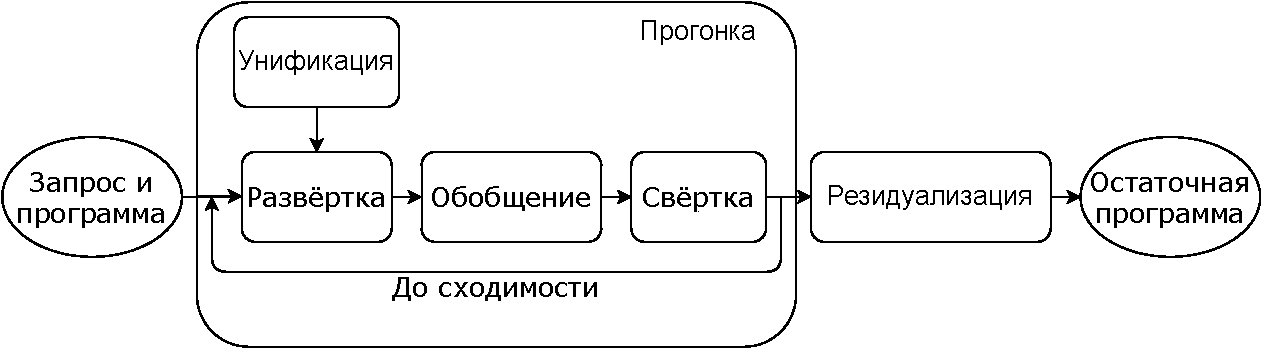
\includegraphics[scale=0.8]{./review/scompflow.pdf}
\caption{Общая схема суперкомпилятора.}
\label{fig:scompScheme}
\end{figure}

% Про "символьное исполнение" https://en.wikipedia.org/wiki/Symbolic_execution
% Сделать ссылку на Ключникова?
%История вычислений представляется в виде {\it графа конфигураций}, где {\it конфигурация}
%описывает состояние вычисления на конкретном шаге. Построение графа происходит на этапе
%{\it прогонки}, во время которого происходит символьное исполнение программы. Потенциально
%такой граф --- который без дополнительных шагов прогонки вырождается в дерево ---
%бесконечный. Для трансформации бесконечного дерева в конечный объект используется {\it cвёртка}
%--- при обработке конфигурации, выражение в которой является {\it переименованием} выражения в одной
%из родительских конфигураций.

История вычислений при суперкомпиляции представляется в виде \emph{графа процессов} --- корневого ориентированного графа,
в котором каждая ветвь --- это отдельный путь вычислений, а каждый узел --- состояние системы или \emph{конфигурация}.
Конфигурация обобщённо описывает множество состояний вычислительной системы или её подсистемы.
% К примеру, конфигурацией можно назвать пару из выражения $1 + x$, которое описывает все возможные суммы с $1$
% свободной переменной $x$, и множество органичений $\{ x \neq 10, x = 1 + x_1 \}$,
% которое сужает множество описываемых состояний до необходимого.
К примеру, конфигурацией можно назвать выражение $1 + x$, в котором параметр $x$ пробегает
все возможные значения своего домена (допустим, множество натуральных чисел) и задаёт
таким образом множество состояний программы\cite{turchinSC}.

Процесс построение графа процессов называется \emph{прогонкой}~\origin{driving}.
Во время прогонки производится шаг символьных вычислений, после которого
в граф процессов добавляются порождённые конфигурации; множество конфигураций
появляется тогда, когда ветвления в программе зависят от свободных переменных.

В процессе прогонки в конфигурациях могут появляться новые свободные переменные,
которые строятся из исходной конфигурации:
если при вычислении выражения его переменная перешла в другую переменную (к примеру, из-за сопоставления с образцом),
то в итоговую конфигурацию будет подставлена новая переменная и связь старой и новой сохранится в
некоторой \emph{подстановке}.
Подстановка --- это отображение из множества переменных в множество возможно замкнутых термов.
Применение подстановки к выражению заменит все вхождения переменных, принадлежащих её домену,
на соответствующие термы. %\todo{Что-нибудь ещё}

Пример графа процессов представлен на рисунке~\ref{fig:pgraphExample}.
\begin{figure}[h!]
\center
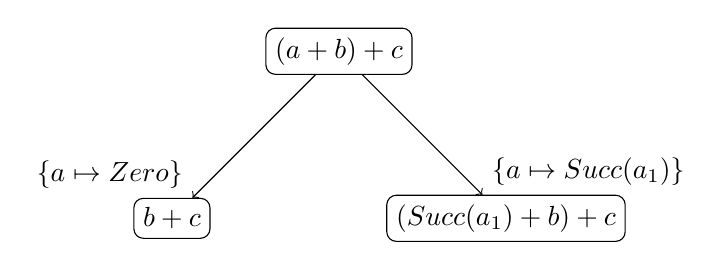
\begin{tikzpicture}[->,node distance=3cm, sibling distance=5cm]
                                                            
  \tikzstyle{conf}=[rectangle,draw, rounded corners=.8ex]

  \node[conf] (root) {$(a + b) + c$} ;
  \node[conf] (childLeft) [below left of = root] {$b + c$};
  \node[conf] (childRight)[below right of = root] {$(\text{Succ}(a_1) + b) + c$};
  \path (root) edge node[above left,pos=1] {$\{a \mapsto \text{Zero}\}$} (childLeft)
        (root) edge node[above right,pos=1]{$\{a \mapsto \text{Succ}(a_1)\}$}(childRight);
\end{tikzpicture}

\caption{Пример части графа процессов.}
\label{fig:pgraphExample}
\end{figure}
Здесь при исполнении выражение $(a + b) + c$, где $a, b, c$ -- натуральные числа,
были рассмотрены возможные значения $a$: это либо оно равно нулю (конструктор Zero), либо это некоторое
число $a_1$, которому прибавили единицу (конструктор Succ). Эти два случая могут задают
различные пути исполнения и, соответственно, добавлены в дерево процессов как два различных состояния,
в одно из которых войдёт программа при исполнении.



Потенциально процесс прогонки бесконечный, к примеру, когда происходят рекурсивные вызовы.
Для превращения бесконечого дерева вычисления в конечный объект, по которому множно
восстановить исходное дерево, используется \emph{свёртка.}

Свёртка~\origin{folding}~--- это процесс преобразования дерева процессов в граф, при котором
из вершины $v_c$ добавляется ребро в родительскую вершину $v_p$,
если выражение в конфигурации в $v_c$ и в $v_p$ равны с точностью до переименования.
Пример ситуации для свёртки изображён на рисунке~\ref{fig:pgraphFoldingExample},
на котором свёрточное ребро изображено пунктиром.

\begin{figure}[h!]
\center
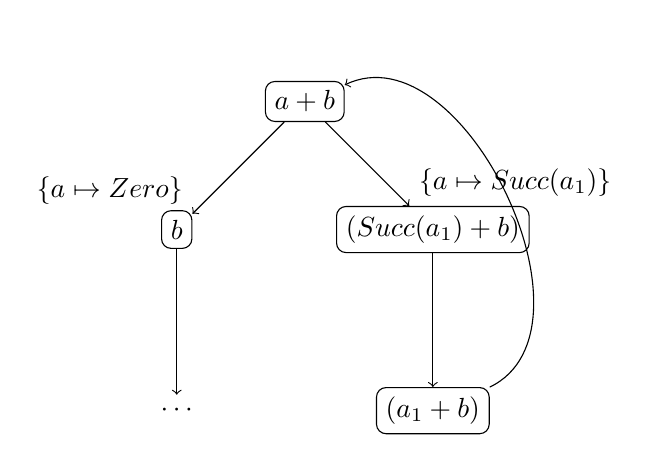
\begin{tikzpicture}[->,node distance=2.3cm, sibling distance=5cm]
                                                            
  \tikzstyle{conf}=[rectangle,draw, rounded corners=.8ex]

  \node[conf] (root) {$a + b$} ;
  \node[conf] (childLeft) [below left of = root] {$b$};
  \node[conf] (childRight)[below right of = root] {$(\text{Succ}(a_1) + b)$};
  \node[conf] (childRight2)[below  of = childRight] {$(a_1 + b)$};
  \node (left)[below of = childLeft] {$\cdots$};

  \path (root) edge node[above left,pos=1] {$\{a \mapsto \text{Zero}\}$} (childLeft)
        (root) edge node[above right,pos=1]{$\{a \mapsto \text{Succ}(a_1)\}$}(childRight)
        (childLeft) edge (left)
        (childRight) edge (childRight2)
        (childRight2) edge[bend right=90] (root);
\end{tikzpicture}

\caption{Пример свёртки.}
\label{fig:pgraphFoldingExample}
\end{figure}

Однако существует ситуации, при котором свёртка не приведёт к тому, что граф превратится в
конечный объект. Такое может произойти, к примеру, когда два выражения структурно
схожи, но не существует переименования, уравнивающих их: $a + b$ и $a + a$.

Для решения этой проблемы используется \emph{обобщение}\cite{scGen}. Обобщение --- это процесс
замены одной конфигурации на другую, более абстрактную, описывающую больше состояний
программы. Для обнаружения ``похожей'' конфигурации используется предикат,
традиционно называемый \emph{свистком}: свисток пробегает по всем
родителям текущей конфигурации и определяет, похожа ли конфигурация на кого-то из них.
В случае, когда свисток сигнализирует о найденной схожести, применяется обобщение.
Сам шаг обобщения может произвести действия трёх видов:
\begin{itemize}
\item \emph{обобщение вниз} приводит к тому, что новая конфигурация заменяет текущую в графе процессов;
\item \emph{обобщение вверх} приводит к замене родительской конфигурации на обобщённую;
\item \emph{разделение}~\origin{split} используется для декомпозиции выражении, элементы которого затем
будут обработаны отдельно.
\end{itemize}
Пример обобщения представлен на рисунке~\ref{fig:pgraphGenExample}

\begin{figure}[h!]
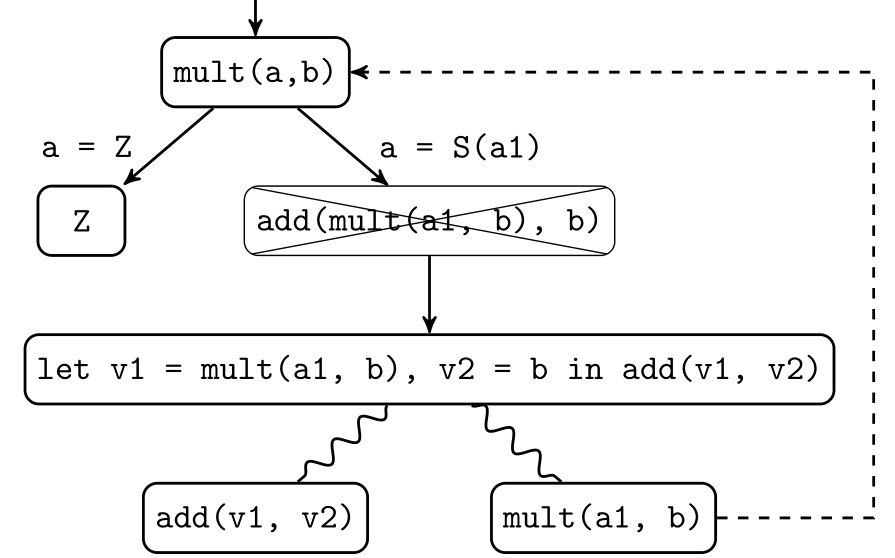
\includegraphics[scale=0.3]{./review/scgenex_temp.png}
\caption{Пример обобщения \todo{свой рисунок}.}
\label{fig:pgraphGenExample}
\end{figure}

Построение программы по графу конфигураций называется \emph{резидуализацией}, а
построенная программа --- \emph{остаточной} \origin{residual}.
Алгоритм выявления остаточной программы основан на обходе дерева, но
в остальном полностью зависит от языка.

% \todo{Написать ещё про СК; продемонстрировать результаты СК; выводы}

Техника суперкомпиляции применяется для функциональных\cite{scHaskell, scPos}
и императивных\cite{scJava} языков. \todo{Кажется, нужны какие-то выводы}

